\documentclass[aspectratio=43]{beamer}
\setbeameroption{show notes on second screen=right}
\usetheme{Boadilla}
\usecolortheme{seahorse}
\usecolortheme{rose}

\usepackage[english]{babel}


\usepackage[utf8]{inputenc}
\usepackage[
  backend=biber,
  style=authoryear,
  sorting=ynt,
]{biblatex}
\addbibresource{myreferences.bib}
\AtEveryBibitem{%
  \clearfield{url}%
  \clearfield{urldate}%
  \clearfield{journaltitle}%
  \clearfield{volume}%
  \clearfield{number}%
  \clearfield{eprint}%
  \clearfield{isbn}%
  \clearfield{issn}%
  \clearfield{pages}%
  \clearfield{pagetotal}%
  \clearfield{day}%,
  \clearfield{note}%
  \clearfield{pages}%
  \clearfield{pmid}%
  \clearfield{pmcid}%
  \clearfield{handle}%
  \clearfield{series}%
  \clearfield{booktitle}%
  \clearfield{maintitle}%
  \clearfield{editor}%
  \clearfield{eventtitle}%
}

\renewbibmacro*{url+urldate}{}
\renewbibmacro*{doi+eprint+url}{\printfield{doi}}

\usepackage{booktabs,xcolor,tabularx}

\author[Mulvihill]{\large Markus Mulvihill}


\title[Thesis Presentation]{Estimating Nonlinear Insulin-Glucose Dynamics in Critically-ill Patients}
\institute[KTH]{\small KTH Royal Institute of Technology}
\date[Aug 2026]{\small August 7th, 2026}
\titlegraphic{
\includegraphics[width=1.5cm]{kthgraphics/KTH-logo.pdf}}
\DeclareMathOperator{\Min}{min}


%\beamerdefaultoverlayspecification{<+->}

\begin{document}

\begin{frame}
  \titlepage
  \note[item]{Supervisor - Martin Lindström}
  \note[item]{Examiner - Ragnar Thobaben}
  \note[item]{Opponent - Divyayan Day}
\end{frame}
%%%%%%%%%%%%%%%%%%%%%%%%%%%%%%%%%%%%%%%%%%%%%%%%%%%%%%%%%%%%

%%%%%%%%%%%%%%%%%%%%%%%%%%%%%%%%%%%%%%%%%%%%%%%%%%%%%%%%%%%%


\AtBeginSubsection[]
{
  \begin{frame}<beamer>{Outline}
    \tableofcontents[currentsection,currentsubsection]
  \end{frame}
}

\section{Motivation}

\subsection{The Fundamental Problem Addressed}
\begin{frame}
  \frametitle{Stress Hyperglycaemia in ICU Patients}
  \begin{figure}
    \centering 
    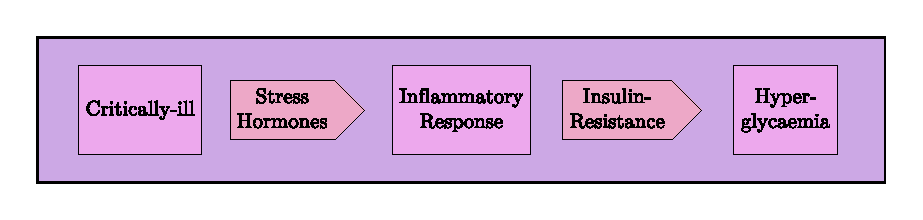
\includegraphics[width=0.96\linewidth]{kthgraphics/problem.pdf}
    \end{figure}
  \note[item] {Inflammatory response secretes stress hormones}
  \note[item] {Acute myocardial infarction, sepsis, stroke}
  \end{frame}

\begin{frame}
     \frametitle{Addressing Hyperglycaemia}
     \begin{columns}[t]
      \begin{column}{0.48\linewidth}
        \begin{itemize}
            \item \textbf{Problem}: \\
            \visible<2->{Stress-induced hyperglycaemia \alert{increases} the likelihood of \alert{mortality}.} \\
        \end{itemize}
      \end{column}
      \begin{column}{0.48\linewidth}
        \begin{itemize}
          \item \textbf{A solution}: \\
          \visible<3->{Maintaining glycaemic levels to 4-6 mmol/L reduced mortalities by 50\% \parencite{berghe_intensive_2001}.}
        \end{itemize}
      \end{column}
     \end{columns}
\end{frame}

\begin{frame}
  \frametitle{Limitations of Intensive Insulin Therapy}
  \begin{columns}
    \begin{column}{0.48\linewidth}   
        \begin{figure}
          \centering
          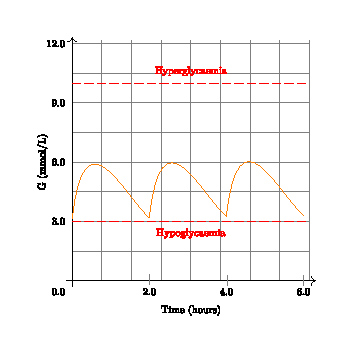
\includegraphics[width=0.96\linewidth]{kthgraphics/example.pdf}
          \caption{Tightly Controlled Blood Glucose}
        \end{figure}
    \end{column}
    \begin{column}{0.48\linewidth}
      \begin{itemize}
        \item<1-> \textbf{What}: \\
         \only<2->{Poor patient adaptability results in cases of \alert{hypoglycaemia} and \alert{high glycaemic variation}. \\}
        \note<3->{Infrequent measurements, not considering nutrition, and not complex to monitor dynamics changes in patient health}
        \item<1-> \textbf{Why}: \\
        \only<3->{Solely utilizing insulin infusions struggles to address patient variability. \\}  
      \end{itemize}
    \end{column}
  \end{columns}
\end{frame}

\begin{frame}
  \frametitle{Role of Model-based Glycaemic Control}
  \begin{itemize}
    \item \textbf{Maybe do a nice photo showing how to convert insulin to equations instead of this long boring text}
    \item<1-> Mathematical formulations of pancreas function provides more insight into glycaemic levels and endogenous insulin production     
    \item<2->\alert{Consequently, physiological models better capture patients' insulin-glucose dynamics to sustain glycaemic ranges} 
    \note[item]<2->{Better method than IIT to be specific}
  \end{itemize}
\end{frame}

\subsection{Previous Work}


\begin{frame}
  \frametitle{Intensive Control Insulin-Nutrition-Glucose (ICING) model}

  \begin{exampleblock}{}
    \citeauthor{lin_physiological_2011} has developed a clinically-validated insulin-glucose model with the following main components
  \end{exampleblock}

  \begin{table}
    \centering
    \small
    \begin{tabularx}{0.96\linewidth}{>{\raggedright\arraybackslash}X l r}
      \toprule
      \textbf{Dynamic}  & \textbf{Notation} & \textbf{Value} \\
      \midrule
      Blood Glucose & $\dot{G}$ & mmol/L \\
      Intersitial Plasma & $\dot{Q}$ & mU/L \\
      Plasma Insulin & $\dot{I}$ & mU/L \\
      Glucose in the Stomach & $\dot{\,P1}$ & mmol \\
      Glucose in the Gut & $\dot{\,P2}$ & mmol \\
      Endogenous Insulin Production & $u_{\,en}(t)$ & mU/min \\
      Insulin Sensitivity & $S_I(t)$ & - \\
      \midrule
      \textbf{Input}  & \textbf{Notation} & \textbf{Value} \\
      \midrule
      Exogenous Insulin & $u_{\,ex}(t)$ & mU/min \\
      Enternal Food & $D(t)$ & mmol/min \\
      Parenteral Glucose & $P_N(t)$ & mmol/min \\
      \bottomrule
    \end{tabularx}
  \end{table}
\end{frame}

\begin{frame}
 \frametitle{Computational Approximation of the ICING model} 
 \begin{itemize}
  \item<1-> The ICING model
 \end{itemize}
\end{frame}

\section{Results and Contributions}

\subsection{Main Results}

\subsection{Key Ideas Behind Implementation}

\section{Summary}

\subsection{Takeaways}

\subsection{Further Reading}
\begin{frame}
  \frametitle{References}
  \printbibliography
\end{frame}


\end{document}
